\documentclass{standalone}
\usepackage{tikz}
\usetikzlibrary{decorations.pathreplacing}
\usepackage{amsfonts}


\begin{document}
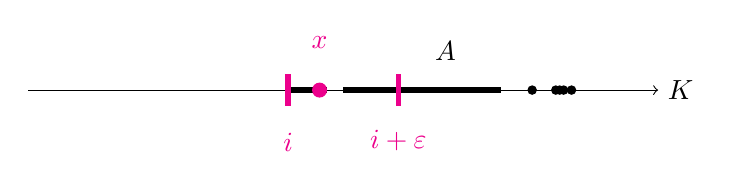
\begin{tikzpicture}
% Draw the real line
  \draw[->] (-4,0) -- (4,0) node[right] {$K$};
  
  % Draw the point 'x' and '0'

 
  \draw[black, line width=2pt] (-0.7,0) -- (-0.2,0);
    \draw[black, line width=2pt] (0,0) -- (2,0);

  \filldraw (2.4,0) circle (1.5pt);
  
  \filldraw (2.7,0) circle (1.5pt);
  \filldraw (2.75,0) circle (1.5pt);
  \filldraw (2.8,0) circle (1.5pt);
  \filldraw (2.9,0) circle (1.5pt);
  
  \node at (1.3, 0.5) {$A$};
  

  \filldraw[magenta] (-0.3,0) circle (2.5pt);
  \node[magenta, anchor=south] at (-0.3,0.4) {$x$};

	
  \node[magenta, anchor=south] at (-0.7,-0.9) {$i$};
  \draw[magenta, line width=2pt] (-0.7,-0.2) -- (-0.7,0.2);
  

 \node[magenta, anchor=south] at (0.7,-0.9) {$i + \varepsilon$};
  \draw[magenta, line width=2pt] (0.7,-0.2) -- (0.7,0.2);
 
  
  
  
  \end{tikzpicture}
\end{document}